\documentclass{beamer}
%
% Choose how your presentation looks.
%
% For more themes, color themes and font themes, see:
% http://deic.uab.es/~iblanes/beamer_gallery/index_by_theme.html
%
\mode<presentation>
{
  \usetheme{default}      % or try Darmstadt, Madrid, Warsaw, ...
  \usecolortheme{default} % or try albatross, beaver, crane, ...
  \usefonttheme{default}  % or try serif, structurebold, ...
  \setbeamertemplate{navigation symbols}{}
  \setbeamertemplate{caption}[numbered]
} 

\usepackage[english]{babel}
\usepackage[utf8x]{inputenc}

\title[Economics]{Incentive Reversal}
\author{Eyal Winter}
\institute{HUJI}
\date{2009}

\begin{document}

\begin{frame}
  \titlepage
\end{frame}

\begin{frame}{Introduction}
\begin{itemize}
    \item Incentive are used to change human behaviors. 
    \item General notion that raising incentives drives the efforts of all agents.
    \item In a sequential decision-making process, boosting incentives may lead to fewer agents applying effort.
\end{itemize}
\vskip .5cm
\item Definition: \textbf{Incentive Reversal} occurs when a strict increase in the reward implies that the set of effort exerting agents under the greater reward is a strict subset of effort exerting agents under the lesser reward.
\begin{center}
    \item Formally, V $<$ V' $\implies$ E(V') $\subsetneq$ E(V)
\end{center}
\end{frame}


\section{Introduction}

\begin{frame}{Incentive Reversal in Practice}

\begin{itemize}
  \item As a track team progresses in the NCAA finals, the anchor of a relay race becomes increasingly responsible for recovering lost time.
  
  \item Suppose a family of four rent a car on vacation. As the surcharge for leaving trash in the rental car increases, the person that returns the vehicle becomes more responsible for cleaning the car.
  
  \item In essence, the payoff is a benefit to the agents. It can represent the value of avoiding a negative outcome or obtaining a positive result.

\end{itemize}

\end{frame}

\begin{frame}{Winter's Example}

\begin{itemize}
	\item Let two agents, $A_1$ and $A_2$, act in sequence.

    \item These agents can choose to exert effort at cost, C, or they can shirk their duties.

    \item Effort guarantees success in the agent's task, while shirking results in success with a probability of $\alpha$.

    \item If both agents accomplish their tasks, the Principal will grant a reward of $V_1$ and $V_2$, respectively.
    


\vskip 1cm
For example, assuming A$_1$ exerts effort,
\newline
A$_2$'s net payout given effort = V$_2$ - C 
\newline
A$_2$'s payout given shirk = $\alpha$V$_2$ 

\end{itemize}

\end{frame}
\begin{frame}{Winter's Example Yields Four Outcomes}

\begin{figure}
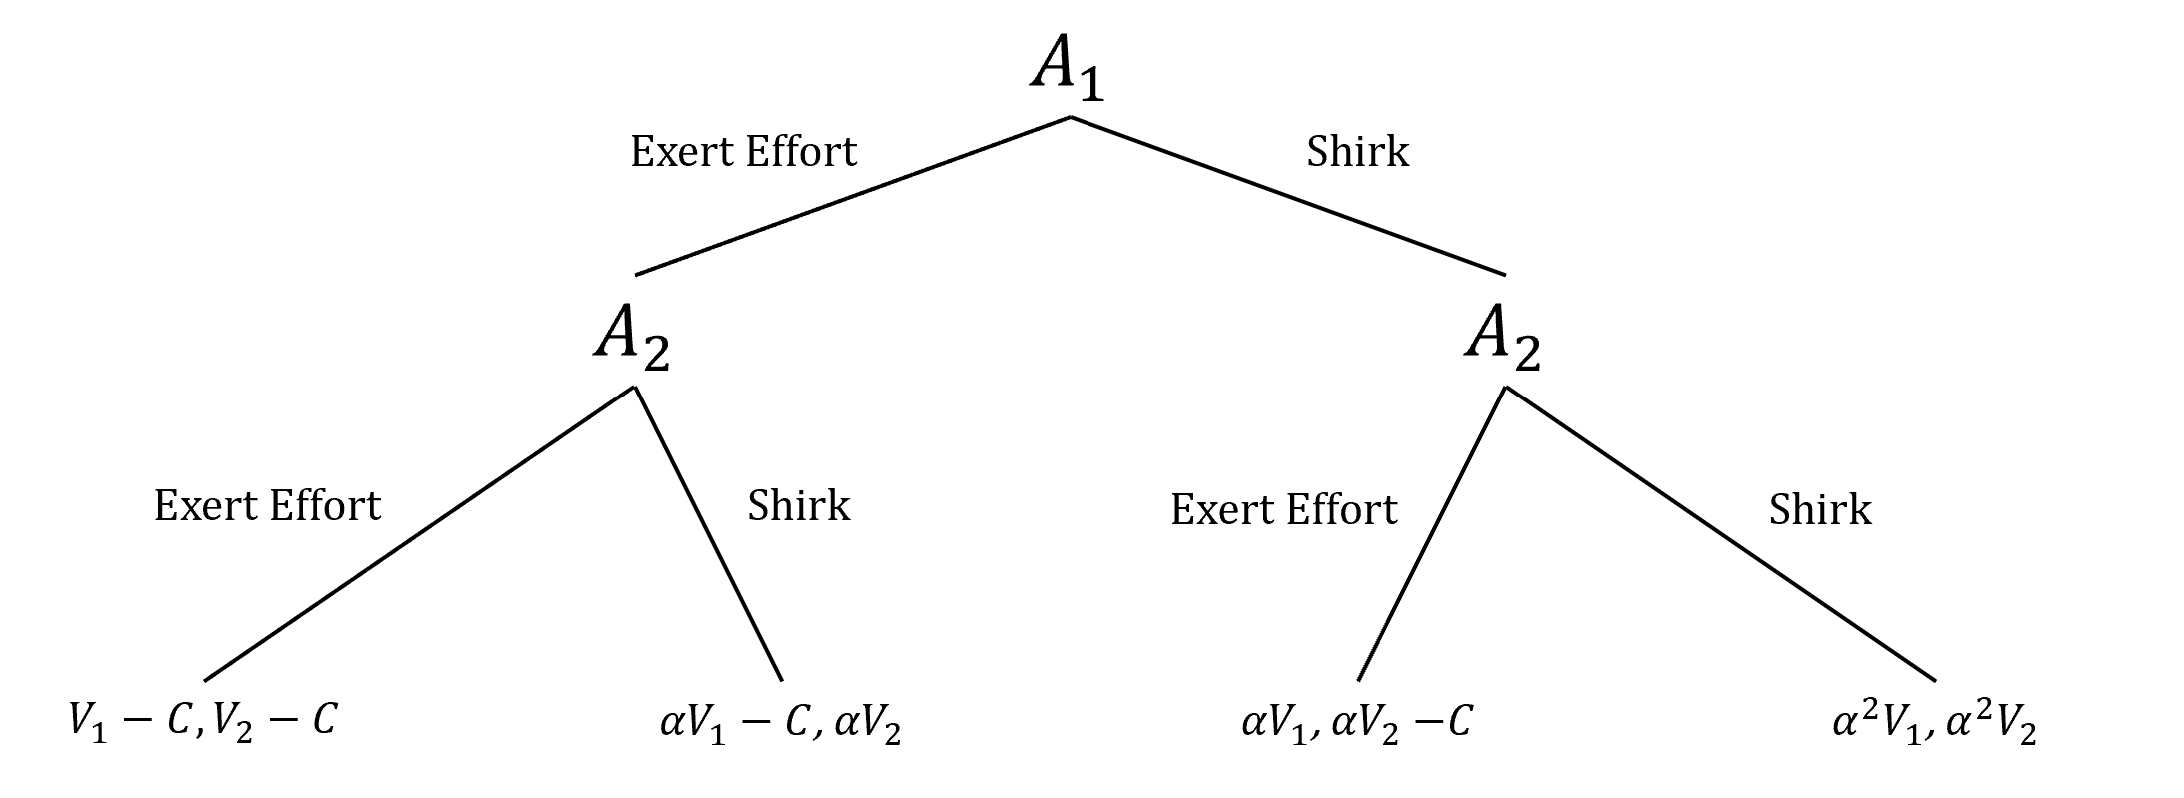
\includegraphics[width=0.75\linewidth]{Winter Game Tree.png}
\end{figure}

\begin{itemize}
    \item Thus, there exists four possible outcomes
\end{itemize}

\begin{center}
    
\begin{bmatrix}

(V$_1$ $-$ C, V$_2$ $-$ C) & ($\alpha$V$_1$, $\alpha$V$_2$ $-$ C)\\
($\alpha$V$_1$ $-$ C, $\alpha$V$_2$) & ($\alpha^2$V$_2$, $\alpha^2$V$_2$) \\

\end{bmatrix}

\end{center}

\end{frame}

\begin{frame}{When and How Incentive Reversal Occurs}
\item The dominant strategy for A$_2$ at some reward vector, V, influences A$_1$'s effort. 
\begin{center}
    
\begin{bmatrix}
(V$_1$ $-$ C, \textbf{V$_2$ $-$ C}) & ($\alpha$V$_1$, \textbf{$\alpha$V$_2$ $-$ C})\\
($\alpha$V$_1$ $-$ C, \textbf{$\alpha$V$_2$}) & ($\alpha^2$V$_1$,  $ \textbf{$\alpha^2$V$_2$}) \\

\end{bmatrix}

\end{center}
    \item Agent 2's dominant strategy is to follow Agent 1 when:
    \begin{itemize}
        \item V$_2$ - C $>$ $\alpha$V$_2$ and $\alpha$V$_2$ - C $<$ $\alpha$$^2$V$_2$  
    \end{itemize}
\item Agent 2's dominant strategy is to always exert effort when:
    \begin{itemize}
        \item $\alpha$V$_2$ - C $>$ $\alpha$$^2$V$_2$ 
    \end{itemize}
\implies \linebreak
\item A$_2$ is indifferent between the two strategies when: \linebreak
$\alpha$V$_2$ - C $=$ $\alpha$$^2$V$_2$ \implies V$_2$ = C$/$($\alpha$ $-$ $\alpha^2$)
\item Therefore, in this example, incentive reversal is contingent upon $\alpha$, C, and V.

\end{frame}

\begin{frame}{Example Computed}

\item Suppose the following values:
\item $\alpha$ = .9
 \item C = 1
 \item V$_1$ = 5.5
 \item V$_2$ = 11
 \item $\implies$ \linebreak
\begin{center}
    
\begin{bmatrix}
(4.5, 10) & (4.95, 8.9)\\
(3.95, 9.9) & (4.46, 8.91) \\

\end{bmatrix}

\end{center}
\begin{itemize}
    \item A$_1$ would be better off shirking if A$_2$ puts in effort. However because A$_2$'s dominant strategy is to follow A$_1$'s behavior and because the 5.33 $>$ 5.127, A$_1$ will not shirk.
\end{itemize}


\end{frame}
\begin{frame}{Principal Raises the Incentive}
Now, suppose the Principal, in an effort to incentivize greater effort, raises V$_1$ and  V$_2$ by 15 percent.
\newline
\item Let: 
\vspace{.001mm}
\item V'$_1$ = 6.33
\vspace{.001mm}
 \item V'$_2$ = 12.6
 \item \implies
\begin{center}
    
\begin{bmatrix}
(5.33, 11.6) & (5.697, 10.34)\\
(4.697, 11.34) & (5.127, 10.206) \\

\end{bmatrix}

\end{center}
\begin{itemize}
    \item Clearly, A$_1$ is still better off shirking if A$_2$ puts in effort, and since A$_2$'s dominant strategy changed to always exert effort, A$_1$ will shirk.
\end{itemize}
 
\end{frame}


\begin{frame}{The Model}

\item Suppose a project with a set n$\in$N agents.
\item Agent \textit{i} can decide to shirk d$_i$ = 0 or put in effort d$_i$ = 1 at a uniform cost of C.
\item Define the function p as the probability that the project succeeds given that \textit{s} number of agents exert effort.
\item The Principal cannot observe the Agents, so a reward vector, V = (V$_1$,..., V$_n$) is established.


\end{frame}

\begin{frame}{The Model 2}

\item T$_i$ denotes the number of agents that make their decision before Agent \textit{i} 

\begin{figure}
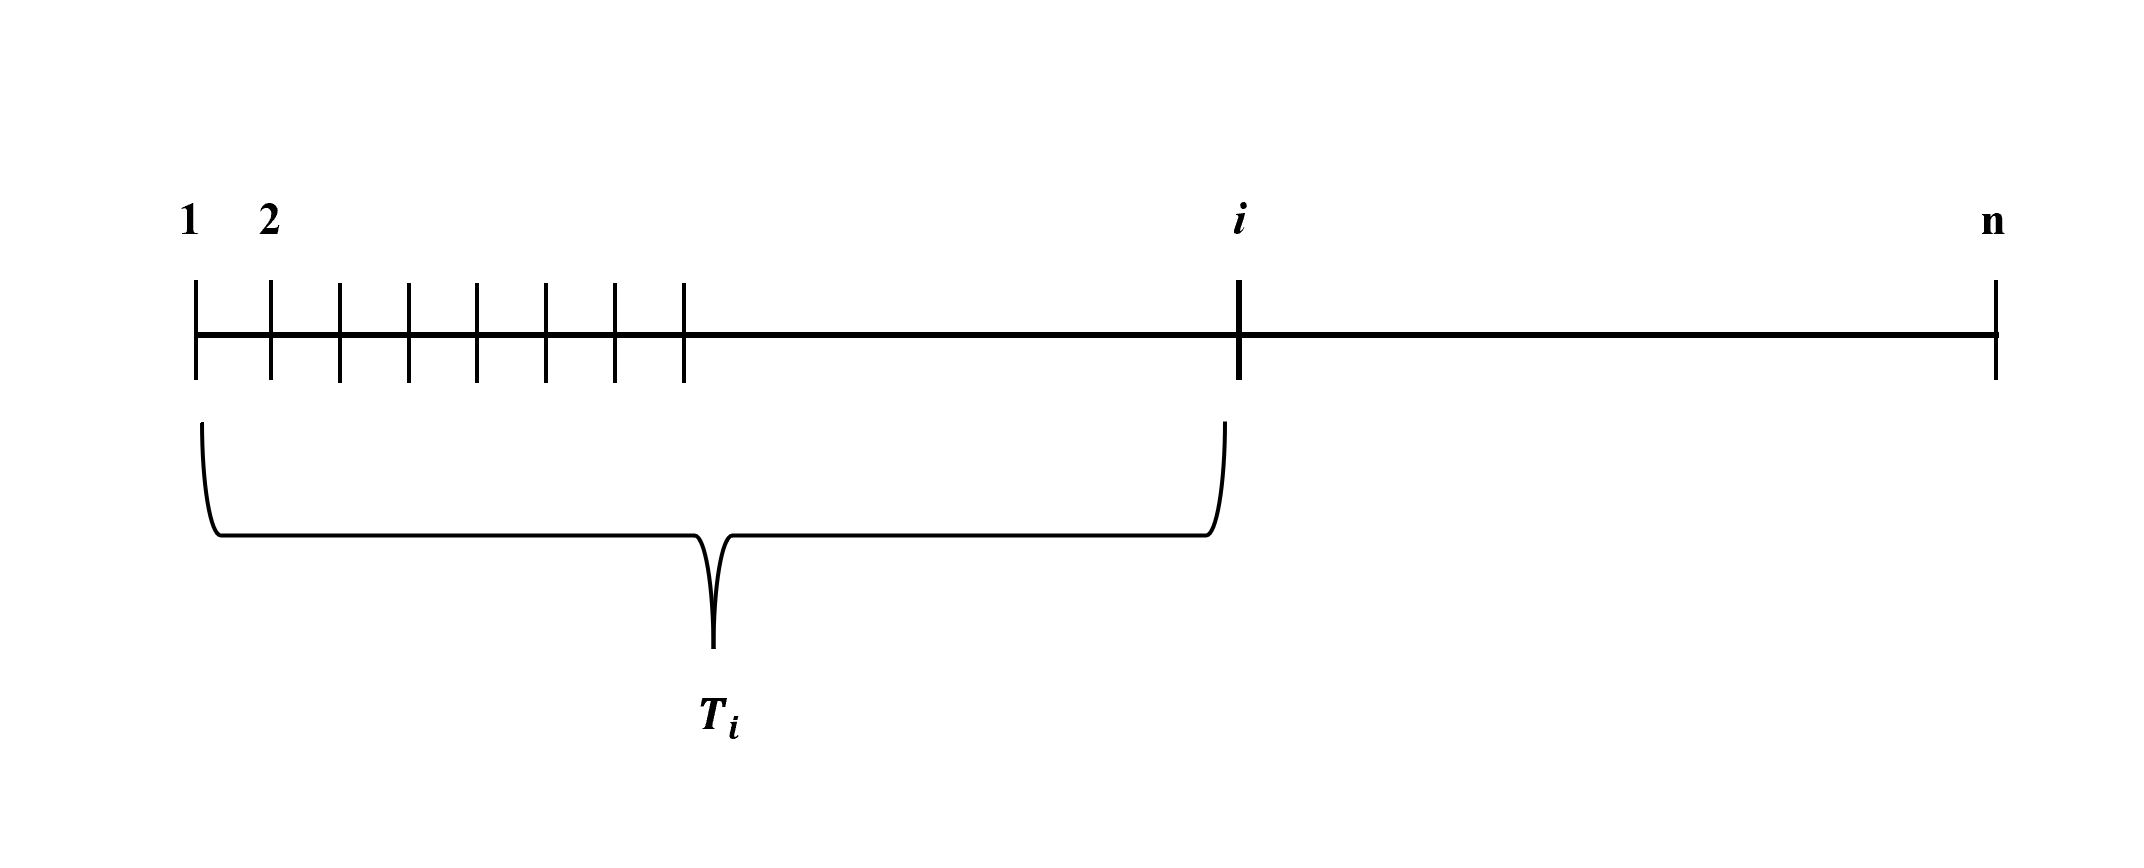
\includegraphics[width=0.5\linewidth]{Set Ti.png}
\caption{This is a visual representation of the set T$_i$.}
\end{figure}
\begin{itemize}

\item Thus, the strategy of \textit{i} can be represented as a function $\sigma$$_i$: 2$^{T_i}$ $\mapsto$ {0,1}
\item This function represents the choice of any agent contingent upon the choices of the preceding decision makers. 

\end{itemize}
\end{frame}

\begin{frame}{The Model 3}

\begin{itemize}
	\item The strategy vector, $\sigma$, contains the strategies for each agent, 
    \item Let E($\sigma$) be the set of all agents that exert effort under $\sigma$ and E(V) be the set of all agents that exert effort with reward V.
    \item Therefore, p(E($\sigma$)) is the probability of success given this strategy vector.
    \item Similar to the prior example, \textit{i}'s reward is a function, f$_i$($\sigma$), of V and P. 
    \end{itemize}
    \vskip .5cm
    \item If \textit{i} $\in$ E($\sigma$), then,  f$_i$($\sigma$) = v$_i$ * p(E($\sigma$)) - C
    \item If \textit{i} $\notin$ E($\sigma$), then,  f$_i$($\sigma$) =  v$_i$ * p(E($\sigma$))
\end{frame}

\begin{frame}{The Model 4}
\item The model relies heavily on technology, \textit{p}, and behavior as the number of effort exerting agents changes. 

\item Recall, p is susceptible to incentive reversal when V $<$ V' $\implies$ E(V') $\subsetneq$ E(V) 


\vskip .5cm
\item Consider: D(\textit{k}) = p(\textit{k+1}) - p(\textit{k}) 
\linebreak

\begin{itemize}
\item \textit{p} demonstrates increasing returns to scale, IRS if D(\textit{k}) is increasing in \textit{k}.  
\begin{itemize}
    \item IRS $\implies$ effort among agents is complimentary.
\end{itemize}
\item \textit{p} demonstrates decreasing returns to scale DRS if D(\textit{k}) is decreasing in k.
\begin{itemize}
    \item DRS $\implies$ effort among agents is a substitute.
\end{itemize}
\end{itemize}
\item In reference to the earlier example, the two-agent situation can only have IRS or DRS.
\end{frame}

\begin{frame}{The Two-Agent Case}
\begin{itemize}
    \item Under n = 2, complementarity (IRS) is necessary and sufficient for inventive reversal.
    \item Proposition 1: p is susceptible to reverse incentive $\iff$ IRS 
    \vskip 5mm
    \begin{itemize}
        \item Lemma 1: If E(V') $\subsetneq$ E(V), then E(V') cannot be (1,1) $\implies$ E(V') = (1,0), (0,1), or (0,0).
        \vskip 5mm
        \item Lemma 2: p satisfies IRS $\implies$ p is susceptible to reverse incentive
    \end{itemize}
\end{itemize}
\vskip .5cm 
\item The proof of Lemma 1 demonstrates that reversal implies A$_2$'s strategy is to match A$_1$ under low vector incentives. 
\vskip 3 mm
\item Lemma 2's proof shows that producing reversal necessitates changing A$_2$'s dominant strategy from always exerting effort to exerting effort $\iff$ A$_1$ exerts effort. 
\end{frame}

\begin{frame}{The Two-Agent Case (Extension)}
\item Relaxing the assumptions in the prior example, let the probability of accomplishing an agent's task, given the agent applies effort, is $\beta$.
\begin{itemize}
    \item Let d $=$ 1 \implies p(success) $=$ $\beta$ $>$ $\alpha$
\end{itemize}
\begin{center}
    
\begin{bmatrix}
($\beta^2$V$_1$ $-$ C, $\beta^2$V$_2$ $-$ C) & ($\beta\alpha$V$_1$, $\beta\alpha$V$_2$ $-$ C)\\
($\beta\alpha$V$_1$ $-$ C, $\beta\alpha$V$_2$) & ($\alpha^2$V$_1$, $\alpha^2$V$_2$) \\

\end{bmatrix}
\end{center}
\item Agent 2's dominant strategy is to follow Agent 1 when:
    \begin{itemize}
        \item $\beta^2$V$_2$ $-$ C $>$ $\beta\alpha$V$_2$, which suggests that the decision rule is never (1,0).
        \item $\beta\alpha$V$_2$ - C $<$ $\alpha$$^2$V$_2$ 
    \end{itemize}
\item Agent 2's dominant strategy is to always exert effort when:
    \begin{itemize}
        \item $\beta\alpha$V$_2$ - C $>$ $\alpha$$^2$V$_2$ 
    \end{itemize}
    Thus, holding V$_2$ and C constant, A$_2$ is indifferent between the two strategies when $\beta$ = ($V$_2$ * $\alpha^2 $+$ C)/{$\alpha$}


\end{frame}
\begin{frame}{Alpha vs Beta}
\begin{itemize}
    \item Plotting this strategic indifference shows the feasible arrangements of $\beta$ and $\alpha$ under given parameters that can generate incentive reversal.
\end{itemize}
    \begin{figure}
        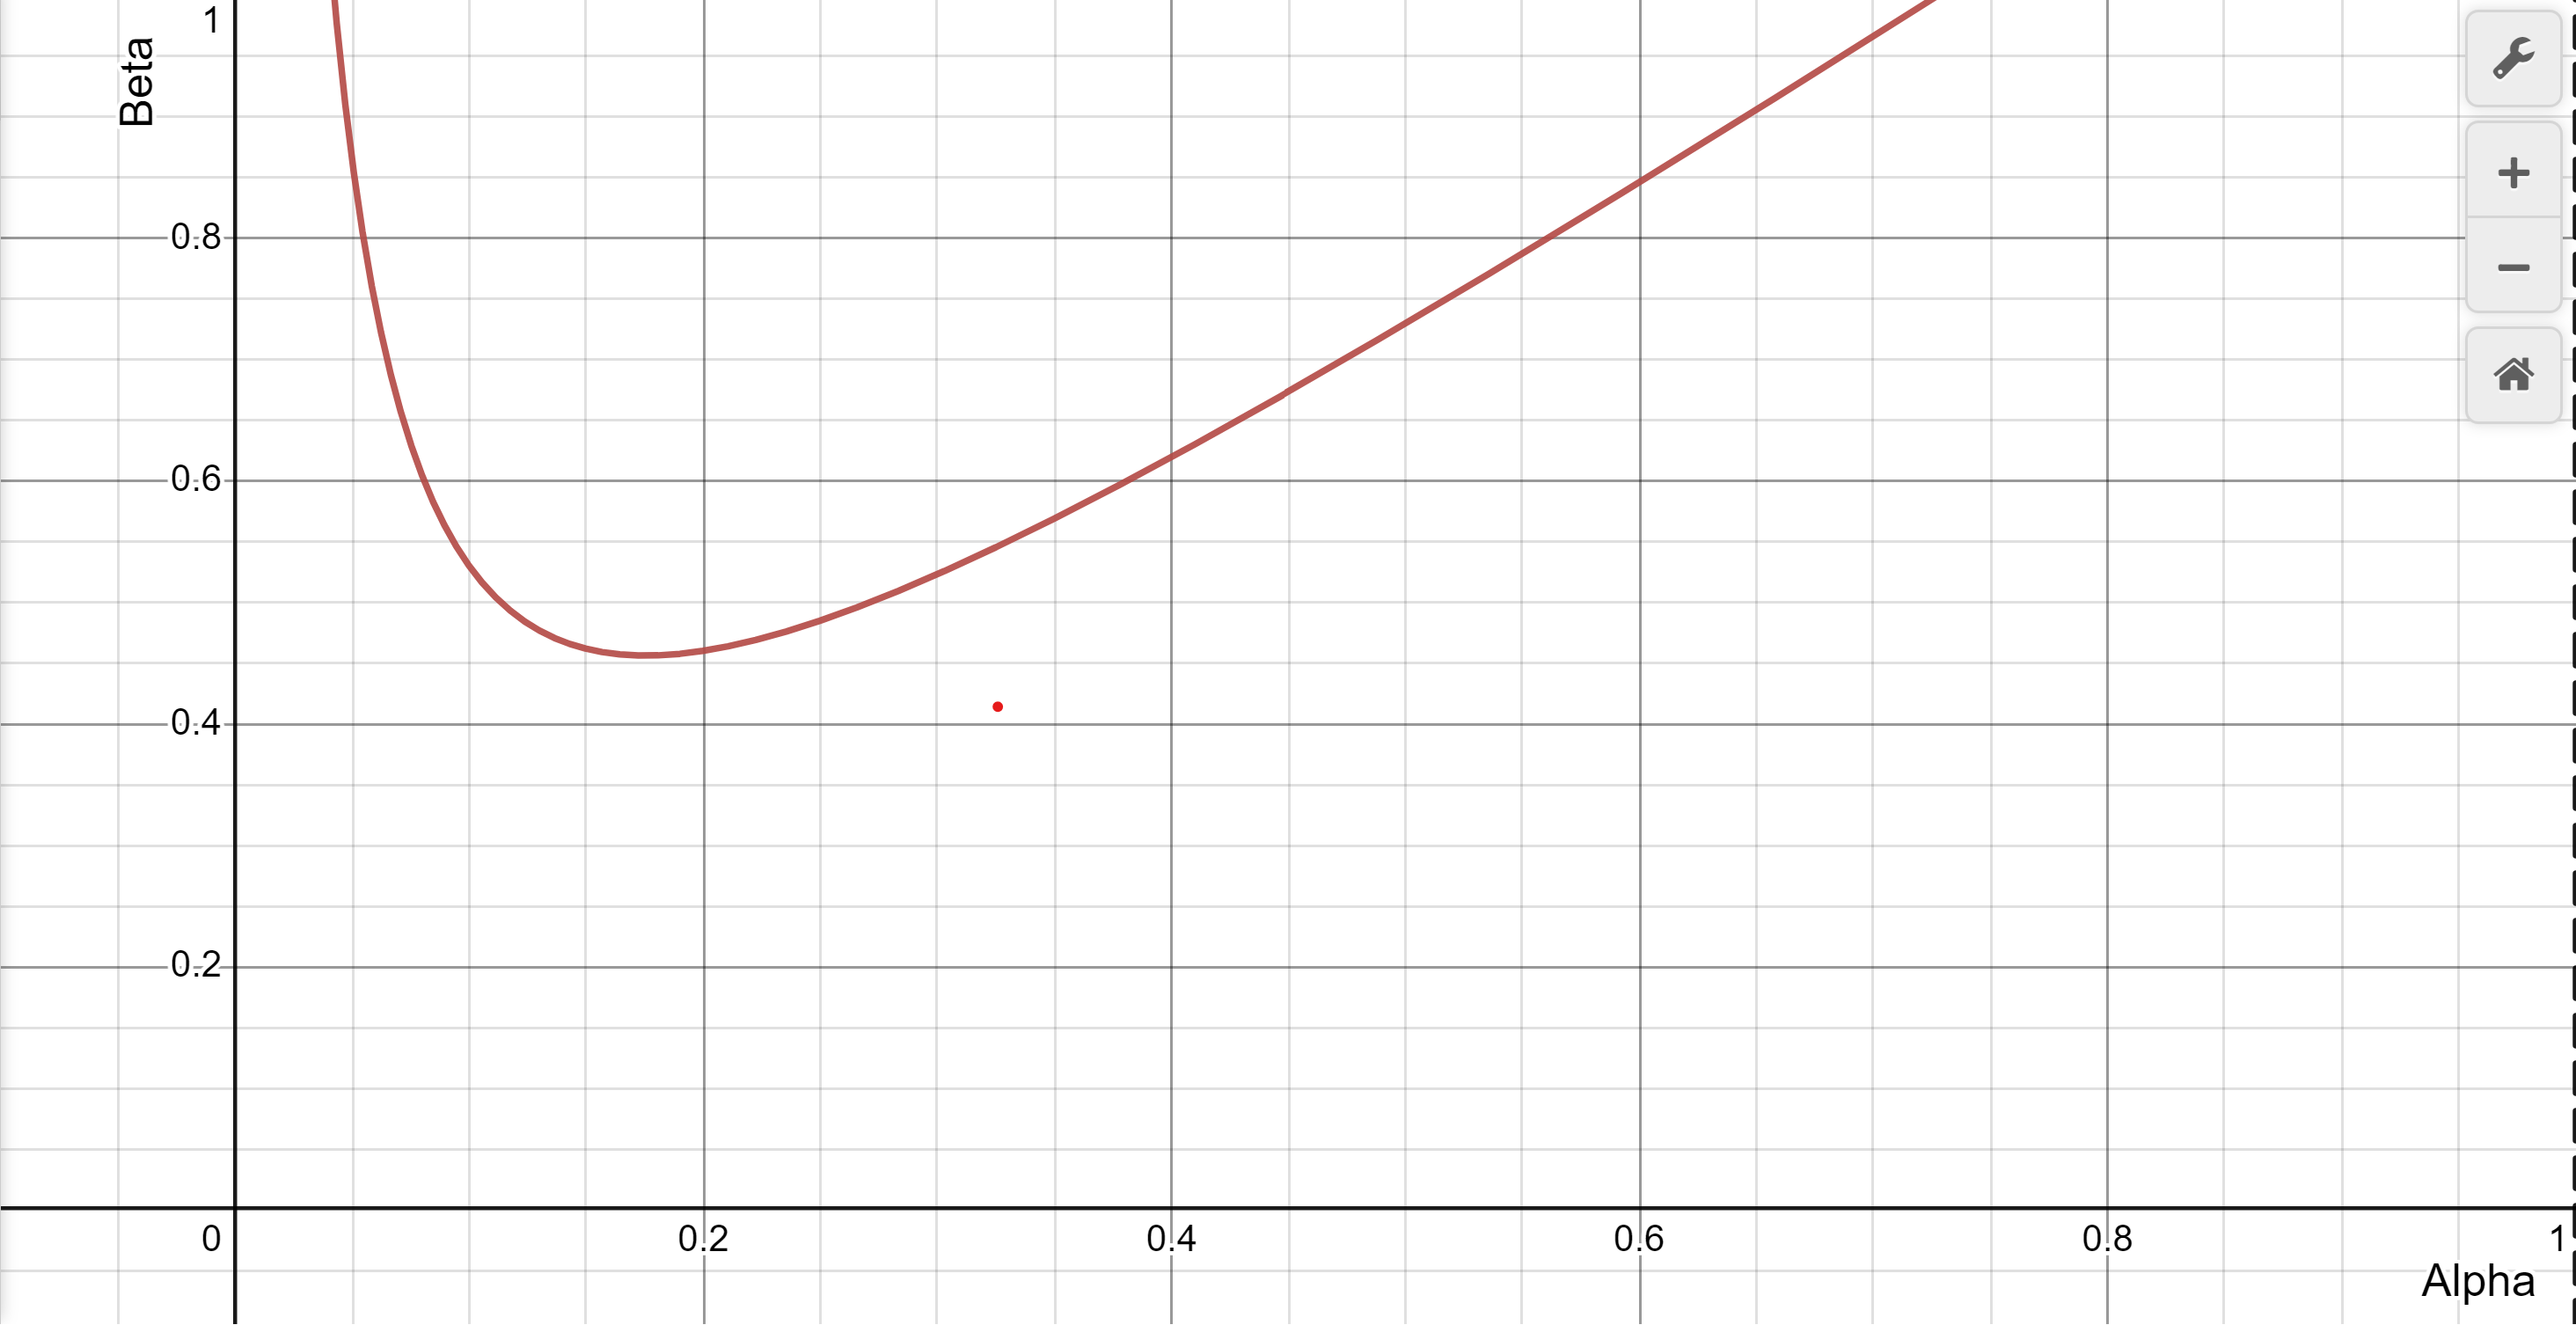
\includegraphics[width=0.75\linewidth]{Better Beta vs Alpha.png}
        \caption{Set C $=$ .04 and V$_2$ $=$ 1.3} 
    \end{figure}
    

\end{frame}

\begin{frame}{Alpha vs Beta Continued}
\begin{figure}
        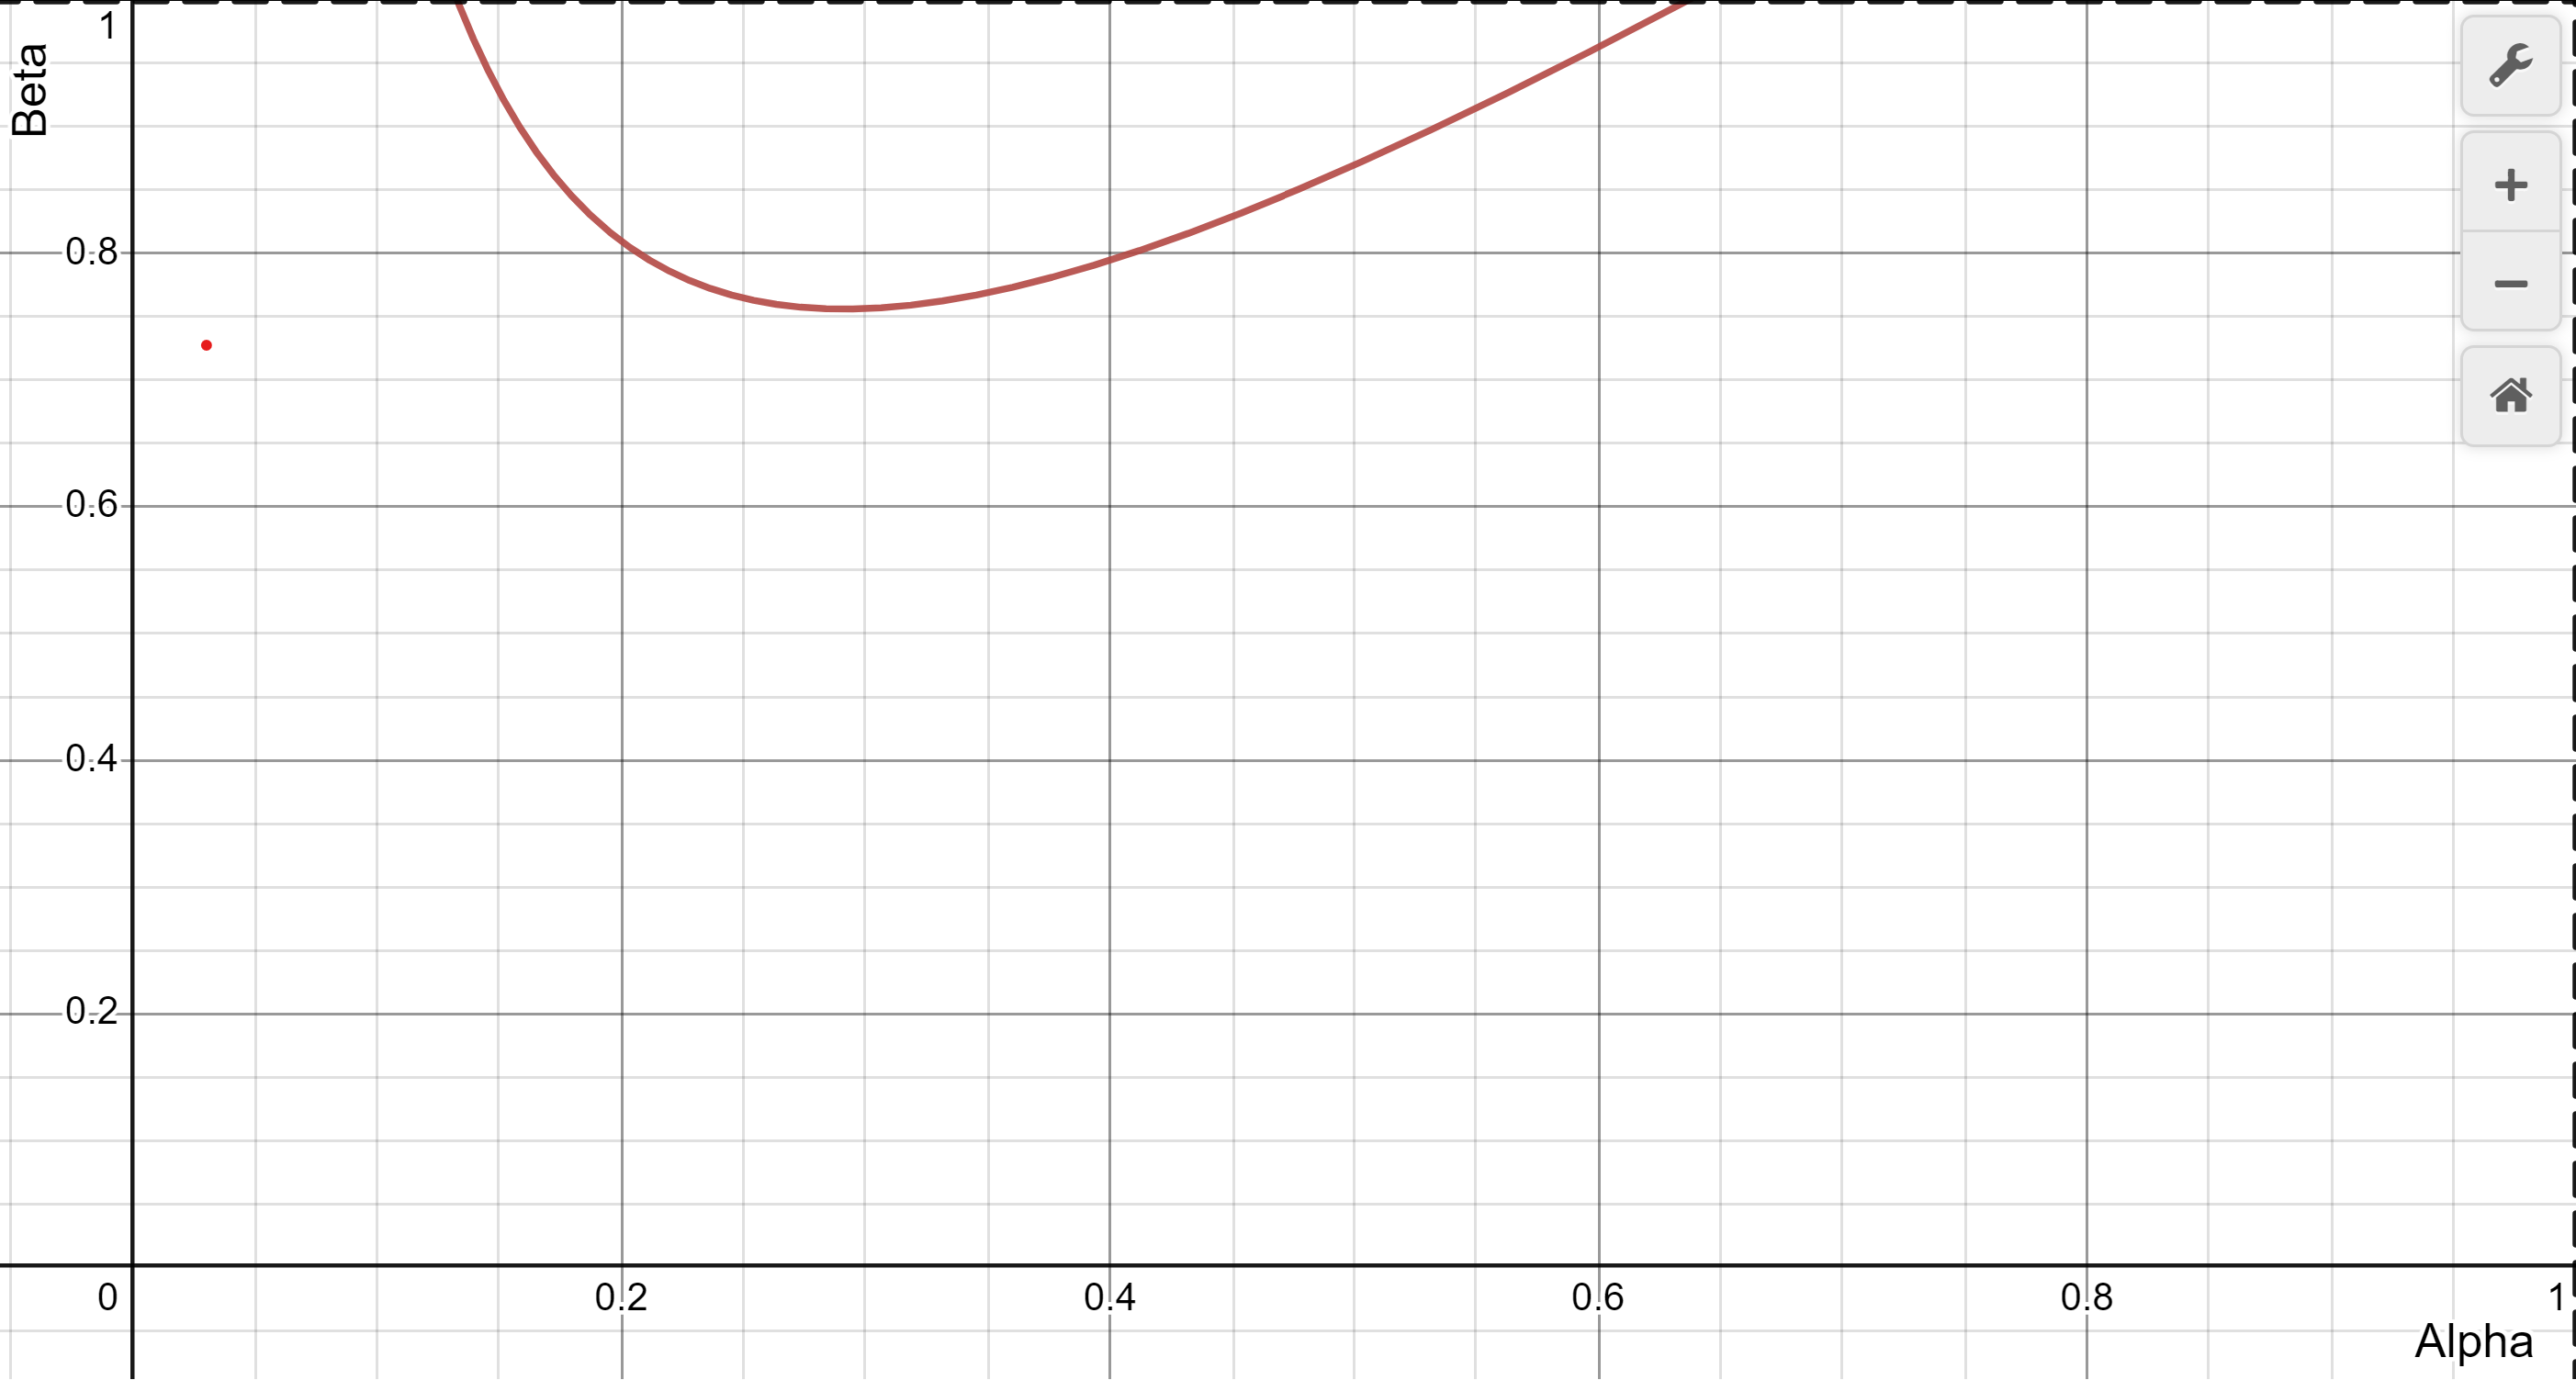
\includegraphics[width=0.5\linewidth]{Increase in C.png}
        \caption{Set C $=$ .11 and V$_2$ $=$ 1.3} 
    \end{figure}

\begin{figure}
        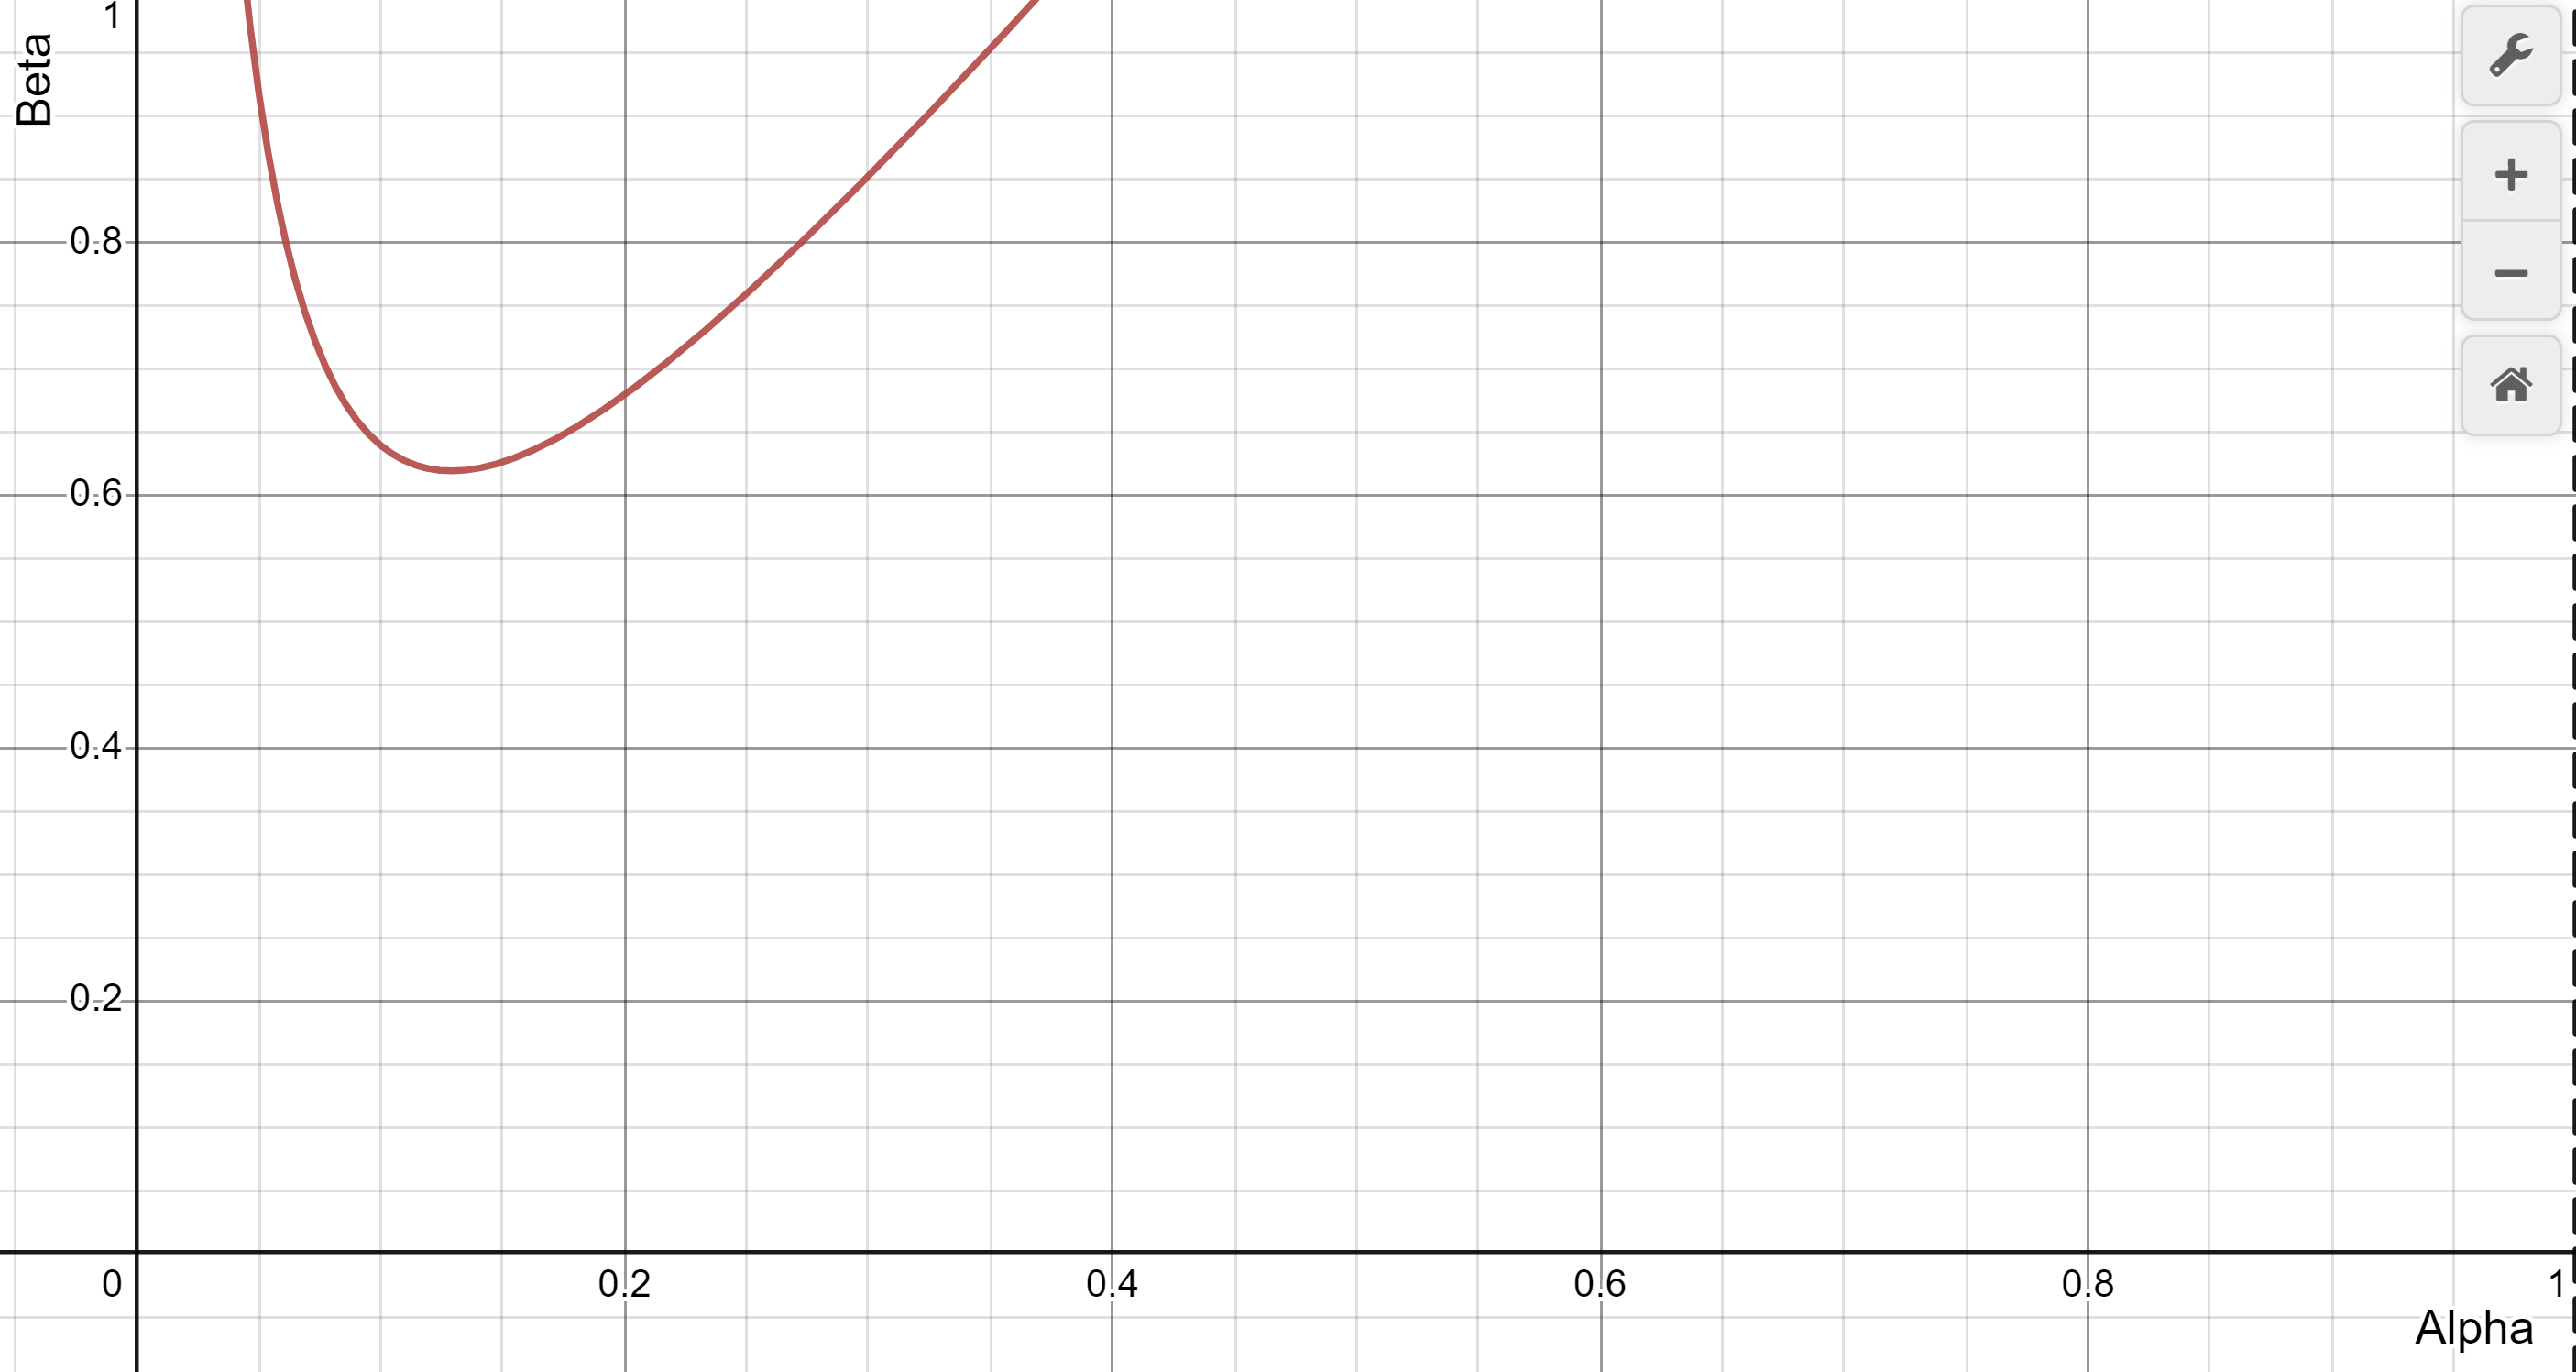
\includegraphics[width=0.5\linewidth]{increase in V2.png}
        \caption{Set C $=$ .04 and V$_2$ $=$ 2.4} 
    \end{figure}
\end{frame}

\begin{frame}{The General Case}
\item In the instance of n agents, some claims are relaxed.
\begin{itemize}
    \item Theorem 1: p is only immune to reversal $\iff$ DRS.
    \item Proposition 2: If a technology has IRS, $\exists$ V $<$ V' s.t. $E(V) = n$ and E(V') contains only one agent.
    \item Proposition 3: If p is $\neg$DRS, then E(V') $\subsetneq$ E(V).
    \item Agents have rational reactions to the effort and shirking of their peers and account for technology. 
\end{itemize}
\end{frame}

\begin{frame}{Key Assumptions}
\item Winter's model makes a few key assumptions. 
\begin{enumerate}
    \item Decisions are made in sequence.
    \item All agents in the game have perfect information of the others' decisions.
    \item  Failure results in zero payment.
    \item Agents have rational reactions to the effort and shirking of their peers and account for technology. 
\end{enumerate}
\end{frame}

\end{document}


